% cap3.tex

\chapter{Desarrollo Metodológico} \label{c3} % la etiqueta para referencias


\section{Replicación del Modelo original y resolución por medio de MCP}

Una de las formas de resolver el problema original de \citeB{amigo_two_2021}, gracias a su forma, es transformarlo en un MCP. Esto es posible gracias al teorema de Karush-Kuhn-Tucker \ref{descripcionkkt} y sus condiciones resultantes. 
\vspace{2.5mm}

Por lo tanto, para replicar el modelo original, se realiza esta transformación y luego es probada en un \textit{solver} para evaluar y comparar sus resultados con el original.

\subsection{MCP problema del productor}

Primero, es necesario aplicar el teorema de KKT en  el problema del productor \ref{fo:prod} para transformarlo en un MCP.
\vspace{2.5mm}

El lagrangeano del problema del productor queda: 

\footnotesize{
\begin{align}
&\mathcal{L}_i(x_i,Q_i,A_i,P_i,V_i) = f_i \big( \pi^d(0),Q_i(0)\big)+ A_i \pi^{a} + I_i x_i(0)  +& \nonumber \\ 
&\sum_{\omega} Pr(\omega)\Bigg[ \sum_{t>0} \frac{1}{(1+R)^t} \Big[ TC_i(t)\cdot f_i \big( \pi^d(t,\omega),Q_i(t,\omega) \big) + TCR_i(t) \cdot I_i\cdot x_i(t,\omega) \Big] + \pi^v(\omega)\cdot \big(P_i(\omega)-V_i(\omega)\big) \Bigg]   + &\nonumber \\
&\kappa_{i}\Big[Q_i(0) -  \big(CF_i\cdot\tau \big)\bar{Q}_i \Big] +\sum_{\omega,t>0} \alpha_{i,\omega,t}\Bigg[Q_i(t,\omega) - \big(CF_i \cdot\tau\big) \big(\bar{Q}_i + \sum_{t^{\prime} \leq t } x_i(t,\omega) + x_i(0) \big)\Bigg] + & \nonumber \\ &\sum_{\omega}\beta_{i,\omega}\Big[V_i(\omega)-A_i \Big] + \sum_{\omega}\gamma_{i,\omega} \Big[-A_{i} - P_{i}(\omega) + V_i(\omega) +\sum_{t>0} Q_i(t,\omega) \varepsilon_{i} + Q_i(0)\varepsilon_{i}\Big] - \sum_{\omega, t>0}\delta_{i,\omega,t} Q_i(t,\omega) + & \nonumber \\ &\sum_{\omega}\psi_{i,\omega} \Big[  \bar{Q}_i+ x_i(0) + \sum_{t > 0} x_i(t,\omega) - RP_i \Big] - \lambda_{i}\Big[Q_{i}(0)\Big] - \sum_{\omega, t>0}\varphi_{i,\omega,t} x_i(t,\omega) - \xi_i x_i(0) & \label{eq:lagrange}
\end{align}}

Realizando las derivadas de primer orden se obtienen:

\subsubsection{Derivada parcial respecto a $x_i(0)$}
\footnotesize{
\begin{align}
    \frac{\partial \mathcal{L} }{\partial x_i(0)} = 0 = I_i  + \sum_{\omega}\psi_{i,\omega} -\sum_{\omega, t>0} \alpha_{i,\omega,t}(CF_i\cdot \tau) -\xi_i=0  \qquad \forall \  i \\
    \Leftrightarrow I_i  + \sum_{\omega}\psi_{i,\omega} -\sum_{\omega, t>0} \alpha_{i,\omega,t}(CF_i\cdot \tau) = \xi_i  \qquad \forall \  i 
\end{align}
}

Donde $\xi_i$ es la variable dual en \ref{res:capi0}. Por lo que esta kkt debe ser complementaria a $x_i(0)$, obteniendo la siguiente complementariedad:

\footnotesize{
\begin{align}
    x_i(0)\geq 0 \qquad \forall \  i \\
    I_i  + \sum_{\omega}\psi_{i,\omega} -\sum_{\omega, t>0} \alpha_{i,\omega,t}(CF_i\cdot \tau) \geq 0  \qquad \forall \  i\\
    x_i(0)\cdot(I_i  + \sum_{\omega}\psi_{i,\omega} -\sum_{\omega, t>0} \alpha_{i,\omega,t}(CF_i\cdot \tau))=0 \qquad \forall \  i
\end{align}
}
En el código GAMS , se escribió la kkt de esta complementariedad de la siguiente forma en la línea 654:
\begin{verbatim}
kkt_x_first_producer(i).. Inv(i)*(1+percent(i)) + sum(w, psi(i,w))- CF(i)*t_year
*sum(w, sum( tau2,alpha(i,w,tau2))) - xi(i)=g=0;
\end{verbatim}
Siendo xi(i) la variable dual $\xi_i$ . Donde esta kkt se complementa con la variable respectiva $x_i(0)$ en la línea 724 del código.
\begin{verbatim}
kkt_x_first_producer.x_first
\end{verbatim}

\subsubsection{Derivada parcial respecto a $x_i(t,\omega)$}
\footnotesize{
\begin{align}
    \frac{\partial \mathcal{L} }{\partial x_i(t,\omega)}= 0 = Pr(\omega) \Bigg[\frac{1}{(1+R)^t}TCR_i(t) \cdot I_i \Bigg] - \sum_{t> t\prime}\alpha_{i,\omega,t} ( CF_i \cdot \tau)+ \psi_{i,\omega}-\varphi_{i,\omega,t} \qquad  \forall \  i, \omega, t> 0\\
    \leftrightarrow Pr(\omega) \Bigg[\frac{1}{(1+R)^t}TCR_i(t) \cdot I_i \Bigg] - \sum_{t> t\prime}\alpha_{i,\omega,t} ( CF_i \cdot \tau)+ \psi_{i,\omega}=\varphi_{i,\omega,t} \qquad  \forall \  i, \omega, t> 0
\end{align}
}

Donde $\varphi$ es la variable dual en la restricción \ref{res:capt}, por lo que, para resolver como MCP se tiene la siguiente complementariedad:


\footnotesize{
\begin{align}
    Pr(\omega) \Bigg[\frac{1}{(1+R)^t}TCR_i(t) \cdot I_i \Bigg] - \sum_{t> t\prime}\alpha_{i,\omega,t} ( CF_i \cdot \tau)+ \psi_{i,\omega} \geq 0 \qquad  \forall \  i, \omega, t> 0\\
    x_i(t,\omega) \geq 0 \qquad  \forall \  i, \omega, t> 0\\
    (Pr(\omega) \Bigg[\frac{1}{(1+R)^t}TCR_i(t) \cdot I_i \Bigg] - \sum_{t> t\prime}\alpha_{i,\omega,t} ( CF_i \cdot \tau)+ \psi_{i,\omega})*x_i(t,\omega)=0
\end{align}
}

Al igual que en el caso anterior, el código mantiene la variable dual, se puede ver en la línea 657 del código el KKT respectivo:

\begin{verbatim}
kkt_x_second_producer(i,tau2,w).. ((1/(1+R))**(ord(tau2)))*Prob(w)*Inv(i)*
(1+percent(i))*TCR(i,tau2)- CF(i)*t_year*sum(tau3$(tauAlpha_i(i,tau2,
tau3)),alpha(i,w,tau3)) + psi(i,w) -varphi(i,w,tau2)  =g=0;
\end{verbatim}

Con varphi(i,w,tau2) como la variable dual mencionada $\varphi_{i,\omega,t}$. 


\subsubsection{Derivada parcial respecto a $Q_i(0)$}
\footnotesize{
\begin{align}
    \frac{\partial \mathcal{L} }{\partial Q_i(0)}= 0 =  \big(a_{i}+b_i Q_{i}(0)\big)-\pi^d(0) + \kappa_i  + \sum_{\omega} \gamma_{i,\omega}\varepsilon_i-\lambda_i \qquad \forall \  i  \\
     \leftrightarrow \big(a_{i}+b_i Q_{i}(0)\big)-\pi^d(0) + \kappa_i  + \sum_{\omega} \gamma_{i,\omega}\varepsilon_i = \lambda_i \qquad \forall \  i
\end{align}
}
$\lambda_i$ es la variable dual de la restricción \ref{res:q0}, por lo que, para resolver como MCP se tiene lo siguiente:
\footnotesize{
\begin{align}
    \big(a_{i}+b_i Q_{i}(0)\big)-\pi^d(0) + \kappa_i  + \sum_{\omega} \gamma_{i,\omega}\varepsilon_i \geq 0 \qquad \forall \  i  \\
    Q_i(0) \geq 0 \qquad \forall \  i  \\
    Q_i(0)*( \big(a_{i}+b_i Q_{i}(0)\big)-\pi^d(0) + \kappa_i  + \sum_{\omega} \gamma_{i,\omega}\varepsilon_i)=0 
\end{align}
}
Como en los anteriores, en el código no se despeja la variable dual $\lambda_i$, se mantiene y se programa el MCP respectivo con la variable $Q_i(0)$. Se puede ver en la línea 660 del código de la siguiente forma:

\begin{verbatim}
kkt_q1_producer(i,tau).. (int(i)+C(i)*Q_first(i,tau))-pi_d(tau) + kappa(i,tau) - 
lambda(i,tau)+sum(w,gamma(i,w)*epsilon(i))=g= 0;
\end{verbatim}

Programando la complementariedad en la línea 728:

\begin{verbatim}
kkt_q1_producer.Q_first    
\end{verbatim}


\subsubsection{Derivada parcial respecto a $Q_i(t,\omega)$}
\footnotesize{
\begin{align}
   \frac{\partial \mathcal{L} }{\partial Q_i(t,w)}= 0
   =Pr(\omega)  \frac{1}{(1+R)^t} \bigg( TC_i(t) \big(a_{i}+b_i Q_i(t,\omega)\big ) -\pi^d(t,\omega) \bigg) + \alpha_{i,\omega,\tau} + \gamma_{i,\omega} \varepsilon_{i} -\delta_{i,\omega,t} \qquad  \forall \ i, \omega, t > 0\\
   \leftrightarrow Pr(\omega)  \frac{1}{(1+R)^t} \bigg( TC_i(t) \big(a_{i}+b_i Q_i(t,\omega)\big ) -\pi^d(t,\omega) \bigg) + \alpha_{i,\omega,\tau} + \gamma_{i,\omega} \varepsilon_{i}= \delta_{i,\omega,t} \qquad \forall \ i, \omega, t > 0
\end{align}
}
$\delta_{i,\omega,t}$ es la variable dual de la restricción \ref{res:qt}, al resolverlo como MCP se tiene la siguiente complementariedad:

\footnotesize{
\begin{align}
    Pr(\omega)  \frac{1}{(1+R)^t} \bigg( TC_i(t) \big(a_{i}+b_i Q_i(t,\omega)\big ) -\pi^d(t,\omega) \bigg) + \alpha_{i,\omega,\tau} + \gamma_{i,\omega} \varepsilon_{i} \geq 0 \qquad \forall \ i, \omega, t > 0\\
    Q_i(t,\omega) \geq 0 \qquad  \forall i, \omega, t > 0\\
    (Pr(\omega)  \frac{1}{(1+R)^t} \bigg( TC_i(t) \big(a_{i}+b_i Q_i(t,\omega)\big ) -\pi^d(t,\omega) \bigg) + \alpha_{i,\omega,\tau} + \gamma_{i,\omega} \varepsilon_{i})\cdot  Q_i(t,\omega)= 0 \qquad \forall \ i, \omega, t > 0
\end{align}
}

La línea 662 del código completa la kkt de la siguiente forma: 

\begin{verbatim}
kkt_qtau_producer(i,tau2,w).. 
((1/(1+R))**(ord(tau2)))*Prob(w)*((TC(i,tau2)*(int(i)+C(i)*Q_second(i,tau2,w)))- 
\end{verbatim}
\begin{verbatim}
pi2_d(tau2,w))+alpha(i,w,tau2)+gamma(i,w)*epsilon(i)-delta(i,tau2,w) =g= 0;
\end{verbatim}

Con la complementariedad escrita de la siguiente forma en la línea 729 del código:
\begin{verbatim}
kkt_qtau_producer.Q_second    
\end{verbatim}

\subsubsection{Derivada parcial respecto a $A_i(t)$}
\footnotesize{
\begin{align}
   \frac{\partial \mathcal{L} }{\partial A_i}= 0
   = \pi^{a} - \sum_{\omega}\beta_{i,\omega} - \sum_{\omega}\gamma_{i,\omega}  \qquad \forall \  i \\
\end{align}
}

Para resolverlo como MCP se tiene la siguiente complementariedad:
\footnotesize{
\begin{align}
    \pi^{a} - \sum_{\omega}\beta_{i,\omega} - \sum_{\omega}\gamma_{i,\omega} \geq 0 \qquad \forall  i\\
    A_i \geq 0 \qquad \forall  i\\
    (\pi^{a} - \sum_{\omega}\beta_{i,\omega} - \sum_{\omega}\gamma_{i,\omega}) \cdot A_i = 0 \qquad \forall  i
\end{align}
}

En el código se tiene lo siguiente en la línea 664:
\begin{verbatim}
   kkt_A_producer(i).. pi_a - sum(w, beta(i,w)) - sum(w, gamma(i,w))=g= 0 
\end{verbatim}

Y efectuando la complementariedad en la línea 730:
\begin{verbatim}
    kkt_A_producer.A
\end{verbatim}

\subsubsection{Derivada parcial respecto a $V_i(w)$}
\footnotesize{
\begin{align}
   \frac{\partial \mathcal{L} }{\partial V_i(w)}= 0
   = -Pr(\omega) \pi^v(\omega) + \beta_{i,\omega}  + \gamma_{i,\omega}  \qquad \forall \  i, \omega \\
\end{align}
}

Para resolverlo como MCP se tiene la siguiente complementariedad:
\footnotesize{
\begin{align}
    -Pr(\omega) \pi^v(\omega) + \beta_{i,\omega}  + \gamma_{i,\omega} \geq 0 \qquad \forall \  i, \omega \\
    V_i(w) \geq 0 \qquad \forall  i,\omega \\
    (-Pr(\omega) \pi^v(\omega) + \beta_{i,\omega}  + \gamma_{i,\omega}) \cdot  V_i(w) = 0  \qquad \forall \  i, \omega 
\end{align}
}

Programando la kkt en el código en la línea 667:
\begin{verbatim}
    kkt_V_producer(i,w)..  -Prob(w)*pi_v(i,w)+beta(i,w)+gamma(i,w)=g= 0
\end{verbatim}

Completando la complementariedad en la línea 731:
\begin{verbatim}
    kkt_V_producer.V
\end{verbatim}

\subsubsection{Derivada parcial respecto a $P_i(w)$}
\footnotesize{
\begin{align}
   \frac{\partial \mathcal{L} }{\partial P_i(w)}= 0
   = Pr(\omega) \pi^v(\omega) -\gamma_{i,\omega} \qquad \forall \  i, \omega \\
\end{align}
}

Para resolverlo como MCP se tiene la siguiente complementariedad:
\footnotesize{
\begin{align}
    Pr(\omega) \pi^v(\omega) -\gamma_{i,\omega} \geq 0 \qquad \forall \  i, \omega \\
    P_i(w) \geq 0 \qquad \forall  i,\omega \\
    (Pr(\omega) \pi^v(\omega) -\gamma_{i,\omega}) \cdot  P_i(w) = 0  \qquad \forall \  i, \omega 
\end{align}
}

Programando la kkt en el código en la línea 670:
\begin{verbatim}
    kkt_P_producer(i,j,w)$(ord(j) <> ord(i))..      Prob(w)* pi_v(j,w)-gamma(i,w) =g= 0
\end{verbatim}

Completando la complementariedad en la línea 732:
\begin{verbatim}
    kkt_P_producer.P  
\end{verbatim}

\subsubsection{Completando el problema del productor}
El resto de las complementariedades del problema del productor se producen al complementar las restricciones del modelo original con sus variables duales:

\footnotesize{
\begin{align}
    & 0 \leq \big(CF_i \cdot \tau \big) \Bigg[\bar{Q}_i + \sum_{t\leq t^{\prime}} x_i(t,\omega) + x_i(0) \Bigg] - Q_i(t,\omega)  \perp \alpha_{i,\omega,\tau} \geq 0 \qquad \forall \ i, \omega, t  > 0\\
    & 0 \leq \Big(CF_i\cdot\tau \Big)\bar{Q}_i(0)-Q_{i}(0) \perp \kappa_i \geq 0 \qquad \forall \ i \\
    & 0 \leq  A_{i} - V_i(\omega) \perp \beta_{i,\omega} \geq 0 \qquad \forall  \ \omega \\
    & 0 \leq  A_{i} + P_{i} (\omega) - V_i(\omega) - \sum_{t>0} Q_i(t,\omega) \varepsilon_{i} -Q_i(0)\varepsilon_{i} \perp \gamma_{i,\omega} \geq 0 \qquad \forall \ i, \omega\\
    & 0 \leq  RP_i - \bar{Q}_i - x_i(0) - \sum_{t>0} x_i(t,\omega) \perp \psi_{i,\omega} \geq 0 \qquad \forall \ i,\omega 
\end{align}
}
Las cuales se encuentran programadas entre las líneas 609 y 703 del código:

\begin{verbatim}
    capacity_stage_2_xnext(i,w,tau2).. CF(i)*t_year*(sum(tau3$(tau3_i(i,tau2,tau3)),
    x_next(i,tau3,w))+x_first(i)+Q_barT2(i,tau2) +Q_bar(i))-Q_second(i,tau2,w) =g=0;
\end{verbatim}
\begin{verbatim}
    capacity_stage_1(i,tau)..  CF(i)*t_year*Q_bar(i)- Q_first(i,tau) =g=0;
\end{verbatim}
\begin{verbatim}
    trading_permits(i,w)..  A(i)-V(i,w) =g= 0;
\end{verbatim}
\begin{verbatim}
    total_allowances(i,w)..  A(i) + sum(j$(ord(j) <> ord(i)),P(i,j,w))-V(i,w) - 
    sum(tau2,Q_second(i,tau2,w)*epsilon(i)) - sum(tau,Q_first(i,tau)*epsilon(i))   =g= 0;
\end{verbatim}
\begin{verbatim}
    resource_potential(i,w)..   -Q_bar(i) - x_first(i) - sum(tau3,x_next(i,tau3,w))+
    sum(tau2,Q_barT2(i,tau2)) + RP(i) =g= 0;
\end{verbatim}

Existiendo sus complementariedades entre las líneas 734 y 744:

\begin{verbatim}
    capacity_stage_1.kappa
    capacity_stage_2_xnext.alpha
    resource_potential.psi
    trading_permits.beta
\end{verbatim}

\subsection{MCP problema del subastador}

En adición a lo realizado con el problema del productor, se debe transformar el problema del subastador \ref{eq:sub} en un MCP. Al igual que el caso anterior, para convertir el problema en un MCP, una de las opciones es aplicar el teorema de KKT. Para comenzar, se obtiene el siguiente lagrangeano:

\footnotesize{
\begin{align}
\mathcal{L}(\theta) = -\theta\pi^a + \mathcal{F}(\theta) - \eta (\varphi^-1(M)\sigma+\mu-\theta) - \varrho(\theta)  \label{eq:lagrange2}
\end{align}}

\subsubsection{Derivada parcial respecto a $\theta$}

Debido a que $\theta$ es la única variable del modelo, solo se debe realizar la derivada del lagrangeano respecto a esta. Obteniendo lo siguiente:

\footnotesize{
\begin{align}
    \frac{\partial \mathcal{L}(\theta) }{\partial \theta} = 0 =  -\pi^a + \frac{\partial\mathcal{F}(\theta)}{\partial \theta} + \eta - \varrho \\
    \Leftrightarrow -\pi^a + \frac{\partial\mathcal{F}(\theta)}{\partial \theta} + \eta = \varrho \label{kkt:subastadororiginal}
\end{align}
}
Donde $\varrho$ es la variable dual de la naturaleza de $\theta$ (\ref{res:sub2}). Obteniendo la siguiente complementariedad:

\footnotesize{
\begin{align}
    \theta \geq 0 \\
    -\pi^a + \frac{\partial\mathcal{F}(\theta)}{\partial \theta} + \eta \geq 0\\
    \theta \cdot (-\pi^a + \frac{\partial\mathcal{F}(\theta)}{\partial \theta} + \eta)=0
\end{align}
}
En el código GAMS de la programación del modelo, se encuentra la kkt \ref{kkt:subastadororig} en la línea 716:

\begin{verbatim}
    kkt_auctioneer..                         -pi_a + eta  =g=0
\end{verbatim}

Realizando la complementariedad en la línea 756:

\begin{verbatim}
    kkt_auctioneer.theta
\end{verbatim}

Para finalizar el MCP del subastador es necesario considerar la complementariedad de la restricción \ref{res:sub2}, obteniendo lo siguiente: 

\footnotesize{
\begin{align}
 \eta \geq 0 \\
 \varphi^-1(M)\sigma+\mu-\theta \geq 0 \\
 \eta \cdot (\varphi^-1(M)\sigma+\mu-\theta)=0
\end{align}}

Esta restricción y complementariedad se encuentran en las líneas 717 y 757 respectivamente:

\begin{verbatim}
    theta_const..   -theta + PhiRisk*(Std)+mean =g= 0;
    theta_const.eta
\end{verbatim}

\subsection{Condiciones de mercado}
Para lograr unir ambos problemas en un solo MCP es necesario incluir las restricciones de condiciones de mercado \ref{rescom:1}, \ref{rescom:2},\ref{res:3},\ref{rescom:4}. De estas se obtienen las siguientes complementariedades:

\subsubsection{Restricción de permisos disponibles}
\footnotesize{
\begin{align}
 \pi^a \geq 0 \\
 \theta - \sum_{i}A_i = 0  
\end{align}}
En el código se encuentra la restricción y complementariedad en las líneas 708 y 751 respectivamente: 
\begin{verbatim}
    kkt_A_theta..    theta - sum(i,A(i))=e= 0;
    kkt_A_theta.pi_a
\end{verbatim}

\subsubsection{Restricción de equilibrio en el mercado de compra y venta de permisos}
\footnotesize{
\begin{align}
 \pi^v(\omega) \geq 0 \qquad \forall \omega\\
 \sum_{i}P_{i,\omega} - \sum_{i}V_{i,\omega} = 0 \qquad \forall \omega  
\end{align}}
En el código se encuentra la restricción y complementariedad en las líneas 713 y 752 respectivamente: 
\begin{verbatim}
    kkt_P_V(i,w).. V(i,w)=e=sum(j$(ord(j) <> ord(i)),P(j,i,w));
    kkt_P_V.pi_v 
\end{verbatim}

\subsubsection{Abastecimiento de demanda en la primera etapa}
\footnotesize{
\begin{align}
 \pi^d(0) \geq 0 \\
 \sum_{i}Q_i(0) - D(0) = 0   
\end{align}}
En el código se encuentra la restricción y complementariedad en las líneas 710 y 753 respectivamente: 
\begin{verbatim}
    kkt_Q_D_first(tau).. sum(i,Q_first(i,tau))=e=D1(tau);
    kkt_Q_D_first.pi_d
\end{verbatim}

\subsubsection{Abastecimiento de demanda en la segunda etapa}
footnotesize{
\begin{align}
 \pi^d(\omega,t) \geq 0 \qquad \forall \omega,t\\
 \sum_{i}Q_i(t,\omega) - D(t,\omega) = 0 \qquad \forall \omega,t  
\end{align}}
En el código se encuentra la restricción y complementariedad en las líneas 711 y 754 respectivamente: 
\begin{verbatim}
    kkt_Q_D_second(tau2,w)..sum(i,Q_second(i,tau2,w))=e=D2(w,tau2);
    kkt_Q_D_second.pi2_d
\end{verbatim}

\subsection{Resolución del problema y resultados}

Finalmente, para resolver el problema en GAMS, solo se debe completar la información adicional, como parámetros, definición de variables y aplicar las líneas de código necesarias para un MCP en GAMS. Con esto realizado, se obtuvieron los siguientes resultados:
\vspace{2.5mm}

CREAR UNA TABLA CON LOS RESULTADOS DEL GAMS, INCLUIR DISTINTOS CAP, THETA, LOS PRECIOS, PRODUCCIONES. 
TAL VEZ COMPARAR CON LOS RESULTADOS CON JULIA.

\section{Problema del subastador}

Uno de los problemas del modelo original del subastador \ref{eq:sub} es que para simplificar su cálculo en el \textit{solver} y KKT, la distribución normal asociada al $CAP$ presentaba desviación estándar $\sigma$ igual a cero y el único valor representativo del presupuesto era la media $\mu$, dejando de ser realmente una entrada estocástica. 
\vspace{2.5mm}

También, el subastador es representado como un planificador que minimiza el negativo de la utilidad, siendo $-\theta \pi^a$ el ingreso negativo por ventas de los permisos y $F(\theta)$ una función de costo asociado a la producción de energía por carbón. El problema en esto es que parece no explicar con totalidad la importancia del subastador en el problema. Ya que este debe ser un ente que busca maximizar sus beneficios tal cual  lo son las empresas generadoras de electricidad en el sistema pero debe tener restricciones que lo incentiven a emitir la cantidad de permisos correctos, o sea, la cantidad de permisos más cercana al presupuesto de carbono $CAP$ estocástico del sistema.
\vspace{2.5mm}

Entonces, esta es un área de exploración para determinar cuál sería una reformulación del problema del subastador donde exista un incentivo por emitir los permisos adecuados y así los generadores no tengan que pagar precios más elevados de los que deberían ser.
\vspace{2.5mm}

Una forma propuesta es la de incluir la probabilidad de encontrar un $\theta$ adecuado, el cual afecte el ingreso del subastador (la ganancia no se calcula como $p\cdot q$ sino que como $p\cdot q\cdot P$, donde $P$ es una proporción entre $[0,1]$ que representa la precisión). Esta probabilidad esté determinada por la cantidad invertida en acercarse al presupuesto lo más posible, medido como gasto en información. Esto no remplaza al costo social del carbón (SCC por sus siglas en inglés), es un costo adicional.


\section{Racionalidad del Planificador}

El planificador debe elegir el número de permisos $\theta$ a vender en el mercado en $t=0$ a precio $\pi^a$. Para esto es lógico pensar que la elección del número de permisos se debe basar en el beneficio que genera la venta de los permisos. Los ingresos serán dados por $\pi^a\cdot\theta$. Los costos vendrán dados por una función $\mathcal{F}(\theta)$ que representa, usualmente, el Costo Social del Carbon. Adicionalmente, el subastador dispone de un presupuesto de emisiones de $CO_2$ es $CAP\in\mathbb{R}_+$ que es una variable aleatoria. De esta forma el planificador debiera maximizar sus beneficios, $\pi^a\cdot\theta-\mathcal{F}(\theta)$, restringido a vender una cantidad de permisos inferior al presupuesto, $\theta\leq CAP$.
\vspace{2.5mm}

Sin embargo, $CAP$ es una variable aleatoria difícil de estimar. De esta forma, \citeB{amigo_two_2021} se limitan a incluir una restricción probabilística que limita la sobre-emisión de permisos por una probabilidad $\epsilon$ pequeña:

$$Pr(\theta\geq CAP)\leq\epsilon.$$

De esta forma, dada la estructura estocástica de $CAP$ (por ejemplo, distribuida según una normal con media $\mu$ y varianza $\sigma^2$), el problema del planificador se resume por las ecuaciones (9) y (10) de Amigo et alii.
\vspace{2.5mm}

En este trabajo el objetivo principal del planificador social es el grado de precisión con el que se cumple la restricción presupuestaria $\theta\leq CAP$. De esta forma maximizará

$$r\cdot Pr(\theta\leq CAP)-\tilde{\mathcal{F}}(Pr(\theta\leq CAP)),$$ \label{nuevafposible}

Donde $r$ es la valor de cumplir exactamente con el presupuesto, en este caso es el ingreso total de venta de los permisos ($r = \theta \pi^a$) y $\tilde{\mathcal{F}}$ es una función de costo por desempeño de cumplimiento que puede tomar una forma cuadrática:

\begin{equation}
\begin{array}{rrclcl}
    \tilde{\mathcal{F}}(P)=\begin{cases}0,&P\leq d\\c(P-d)^2,&P>d\end{cases}\label{costoperformace}\\
\end{array}
\end{equation}

Donde $d$ es el umbral de desempeño con información pública y $c$ es el costo marginal de adquirir información para mejorar el desempeño en cumplimiento.
\vspace{2.5mm}

Finalmente, se define el \emph{performance} óptimo para el premio ($r = \theta \pi^a$). Donde el \emph{performace} óptimo  se define como $P^*(r) = (C')^{-1}(r)$ de la siguiente forma:

\begin{equation}
\begin{array}{rrclcl}
    P^*(\theta \pi^a) = \begin{cases}\frac{\theta \pi^a}{2c}+d,&\theta \pi^a\leq 2c(1-d)\\1,&\theta \pi^a>2c(1-d)\end{cases}, \label{performaceoptimo}\\
\end{array}
\end{equation}

\section{Reordenando modelo del subastador con función de costo diferenciable}

\citeB{dewan_estimating_2020} propone la opción de agregar una función de costo asociada al \textit{performance}(rendimiento en inglés) de obtener la variable de decisión (en este caso $*\theta*$) lo más cercana a la óptima al invertir en investigación que mejore la estimación de la variable.
\vspace{2.5mm}

Considerando \ref{nuevafposible}, tomando $Pr(\theta\leq CAP) = P$ con $P = $\textit{performance}, la función objetivo del subastador puede reorganizarse de la siguiente forma:

\begin{equation}
\begin{array}{rrclcl}
    \displaystyle \min_{\theta,P} & -\theta \pi^aP + \tilde{\mathcal{F}}(P)+F(\theta)  \label{fo:performance0}\\
\end{array}
\end{equation}

Para completar el problema de optimización se debe definir ciertos supuesto. Para comenzar, se debe definir que factores serán variables y parámetros. Por el momento, se asume que la única variable es $\theta$ y el subastador busca un \textit{performace} mayor al umbral de información pública.  
\vspace{2.5mm}

Entonces, debe identificarse $\tilde{\mathcal{F}}(P)$ de acuerdo a su definición en \ref{costoperformace} cuando se cumple que el \textit{performace} es mayor al umbral de información pública $d$ entonces se define lo siguiente, conociendo los parámetros $c, d$:

$$\tilde{\mathcal{F}}(P)=c(P-d)^2$$ 

De esto se deben definir las restricciones del problema. La primera corresponde a la positividad de $\theta$. 

\begin{equation}
\begin{array}{cl}
    \theta \geq 0 & (\varrho)\label{res:newsub1}
\end{array}
\end{equation}

Para la segunda, se debe aplicar la función de \textit{performance} óptimo para el ingreso \ref{performaceoptimo}. La idea es encontrar una restricción para definir este problema teniendo solo a $\theta$ como variable. Entonces la opción es aplicar la siguiente restricción: 

\begin{equation}
\begin{array}{cl}
    \theta \pi^a\leq 2c(1-d) & (\eta) \label{res:newsub2}
\end{array}
\end{equation}

Con esto el problema del subastador quedaría reformulado de la siguiente manera:

\begin{equation}
\begin{array}{rrclcl}
    \displaystyle \max_{\theta} & \theta \pi^a(\frac{\theta \pi^a}{2c}+d) - c((\frac{\theta \pi^a}{2c}+d)-d)^2  \\\textrm{s.a.}\\
\end{array}
\end{equation}
\begin{equation}
\begin{array}{cl}
    \theta \pi^a\leq 2c(1-d) & (\eta) \label{res:newsub2}
\end{array}
\end{equation}
\begin{equation}
\begin{array}{cl}
    \theta \geq 0 & (\varrho)\label{res:newsub1}
\end{array}
\end{equation}

\subsubsection{Maximizando el rendimiento}

Esta formulación es considerada completa en un contexto donde, al igual que el trabajo original, se quiere maximizar los \textit{allowances} (permisos de contaminación) para la industria generadora. Pero, en esta memoria, se busca reordenar el problema donde el subastador sufra perdidas por su mala gestión, intentando mejorar su rendimiento.
\vspace{2.5mm}

Para lograr lo anterior, es necesario definir el problema tomando como variable de decisión el rendimiento ( \textit{performance}). Con esto, es necesario definir la variable $P$ respecto a $\theta$ para que poder utilizar el problema en el modelo general al incluir a el problema de los productores(generadores de electricidad).
\vspace{2.5mm}

Luego, de \ref{res:newsub2} y \ref{performaceoptimo} se obtiene la siguiente igualdad:

$$P^*(\theta \pi^a) = \frac{\theta \pi^a}{2c}+d$$

Si se despeja $P$ se obtiene su valor respecto a $\theta$:

$$\theta=\frac{(P-d)2c}{\pi^a}$$

Despejando esta variable en \ref{fo:performance0}, se obtiene la siguiente función objetivo:


\begin{equation}
\begin{array}{rrclcl}
    \displaystyle \max_{P} & \frac{(P-d)2c}{\pi^a} \pi^{a}P - c(P-d)^2  \label{fo:3}\\
\end{array}
\end{equation}

La cuál se puede simplificar llegando a lo siguiente:

\begin{equation}
\begin{array}{rrclcl}
    \displaystyle \max_{P} & c(P^{2}-d^{2}) \label{fo:4}\\
\end{array}
\end{equation}

La cuál tiene sentido pero no es aplicable en el trabajo \citeB{dewan_estimating_2020}, ya que según la proposición 4, descrita en \ref{marco:costos}, el problema de maximización debe ser cóncavo. Pero debido a la forma en la que se definió el premio ($r=\pi^{a}\theta$), la concavidad de la función de costo en este caso no transforma \ref{fo:4} en cóncava. Debido a esto, no se puede encontrar un máximo local que sea también un máximo global en el problema que comprueba la proposición 4.
\vspace{2.5mm}

Esto se comprueba en el gráfico INSERTAR GRÁFICO DE MAXIMIZACIÓN NO CONCAVA
\vspace{2.5mm}

Para lograr la concavidad necesaria, se encuentra la posibilidad de incorporar un elemento del problema original del subastador. Con esto, además de cumplir con la proposición 4, se expande el alcance de este trabajo, ya que ahora no solo se está reordenado el problema al aplicar un sistema nuevo de incentivo, si no que, se incorpora el costo mencionado en el trabajo originial de AMIGO llamado Costo Social del Carbón (SCC). Con esto amplía el estudio para definir este costo respecto al rendimiento del subastador.
\vspace{2.5mm}

La primera aplicación de este costo es la de entender que el costo SCC dependerá de los permisos emitidos, ya que a mayor cantidad de permisos, existirá mayor costos asociados al uso del carbón. Por lo que, inicialmente, se  define el SCC como: $F(\theta)= \alpha\theta + \beta$ ($\alpha$,$\beta$ parámetros). 
\vspace{2.5mm}

Luego, la idea es que este costo transforme \ref{fo:4} a una función cóncava, por lo que se debe cumplir lo siguiente:

\begin{equation}
\begin{array}{rrclcl}
    F(\theta)= \alpha\theta + \beta = kP^2 \label{fo:5}\\
\end{array}
\end{equation}

Donde, si $k>c$ (de \ref{fo:4}), se logra una función objetivo cóncava. Obteniendo, luego de reemplazar la variable de permisos $\theta$ por su valor en función del rendimiento $P$, la siguiente función de costo social a incorporar en el modelo:

\begin{equation}
\begin{array}{rrclcl}
    F(\frac{(P-d)2c}{\pi^a})= \alpha\frac{(P-d)2c}{\pi^a} + \beta = kP^2 \label{fo:5}\\
\end{array}
\end{equation}

De la cuál, se deben encontrar los valores de $\alpha$ y $\beta$ que cumplan con la igualdad.

\section{Reordenar KKT subastador Amigo et alii}


Para evaluar el comportamiento del reordenamiento del subastador, es necesario entender como se comporta el modelo al variar los parámetros y comparar los resultados con el modelo original. \vspace{2.5mm}

Para comenzar, se evaluará el comportamiento del modelo al incluir el nuevo costo de rendimiento explicado en \ref{fo:performance0}. Este será evaluado al modelar el sistema como un MCP al aplicar el teorema de KKT con el nuevo costo resolviendo el problema en GAMS. Se resolverán primero al solamente incluir el costo de rendimiento y no considerar restricciones (solo se considera la naturaleza de las variables) y luego se resolverá considerando restricciones adicionales.
\vspace{2.5mm}

Para realizar la evaluación del modelo, se realizará un gráfico con los resultados similar a la figura \ref{fig:fig6}. En esta se grafica la cantidad de permisos vendidos por el productor que produce energía con carbón y su influencia en el precio de mercado de los permisos. Esto representa el impacto que puede tener el modelo en eliminar el carbón como productor.

\begin{figure}[H]
    \centering
    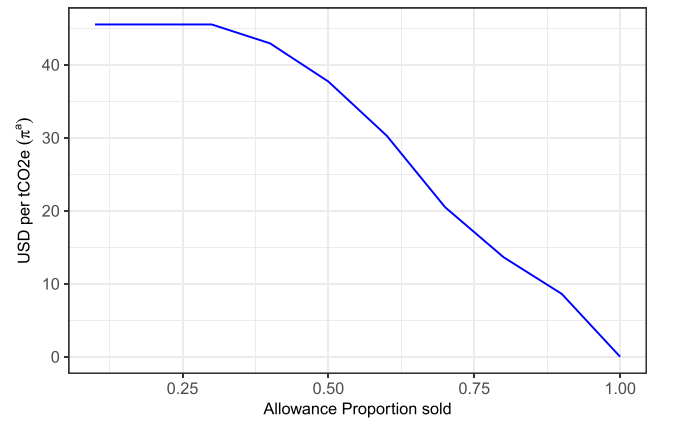
\includegraphics[width=15cm]{docs/DocumentoMemoria/images/figura 6 amigo.png}
    \caption{Venta de permisos por generador de carbón (Fuente: \protect\citeB{amigo_two_2021})}
    \label{fig:fig6}
\end{figure}


\subsubsection{Modelo sin restricciones}

Primero se evaluará el modelo al considerar únicamente la función objetivo del subastador con el costo original $\mathcal{F}$ y el costo de rendimiento. También se considera como variable de decisión únicamente los permisos $\theta$.  

\begin{equation}
\begin{array}{rrclcl}
    \displaystyle \min_{\theta} & -\theta \pi^aP + \tilde{\mathcal{F}}(P)+F(\theta)  \label{fo:perfornorest}\\
\end{array}
\end{equation}
\begin{equation}
\begin{array}{cl}
    \theta \geq 0 & (\varrho)\label{res:sub2}
\end{array}
\end{equation}

Con lo anterior se logra el siguiente Lagrangiano:

$$\mathcal{L}(\theta)=-P\theta\pi^a+\mathcal{F}(\theta)+c(P-d)^2 - \varrho\theta $$

Realizando la derivada de primer orden para $\theta$ se obtiene:

\begin{equation}
\begin{array}{rrclcl}
    \frac{\partial\mathcal{L}(\theta)}{\partial (\theta)}=-P\pi^a+\frac{\partial\mathcal{F}(\theta)}{\partial(\theta)}-\varrho=0 \label{lag1}\\
\end{array}
\end{equation}
\begin{equation}
\begin{array}{rrclcl}
    \rightarrow -P\pi^a+\frac{\partial\mathcal{F}(\theta)}{\partial(\theta)}=\varrho \label{lag1}\\
\end{array}
\end{equation}
Con esto se obtiene la siguiente complementariedad para el problema del subastador:

\begin{equation}
\begin{array}{rrclcl}
    0\leq -P\pi^a+\frac{\partial\mathcal{F}(\theta)}{\partial(\theta)}\perp \theta \geq 0 \label{compllag1}\\
\end{array}
\end{equation}

Al igual que en el modelo original de \citeB{amigo_two_2021}, se consideran los siguientes valores para constantes y parámetros:
\begin{enumerate}
    \item $\frac{\partial\mathcal{F}(\theta)}{\partial(\theta)}=0$
    \item $CAP\sim \mathcal{N}(100MtCO_{2}e,0)$
\end{enumerate}

Con esto, al correr el modelo en el \textit{solver}, cambiando únicamente el valor del rendimiento ($P$), se encontraron los siguientes resultados:

\begin{table}[H]
\centering
\begin{tabular}{|l|l|l|}
\hline
\textbf{P($\%$)} & \textbf{$\theta$ (millones)} & \textbf{$\pi^a$($\frac{\$}{\theta}$)} \\ \hline
0 & N/A & N/A \\ \hline
5 & 104 & 223 \\ \hline
10 & 3203 & 0 \\ \hline
15 & 3203 & 0 \\ \hline
20 & 3203 & 0 \\ \hline
25 & 3203 & 0 \\ \hline
30 & 3203 & 0 \\ \hline
35 & 3203 & 0 \\ \hline
40 & 3203 & 0 \\ \hline
45 & 3203 & 0 \\ \hline
50 & 3203 & 0 \\ \hline
55 & 3203 & 0 \\ \hline
60 & 3203 & 0 \\ \hline
65 & 3203 & 0 \\ \hline
70 & 3203 & 0 \\ \hline
75 & 3203 & 0 \\ \hline
80 & 3203 & 0 \\ \hline
85 & 3203 & 0 \\ \hline
90 & 3203 & 0 \\ \hline
95 & 3203 & 0 \\ \hline
100 & 1870 & 0 \\ \hline
\end{tabular}
\caption{Resultados con rendimiento y sin restricciones}
\label{tabla:sinrestr}
\end{table}


Los resultados encontrados en el Cuadro \ref{tabla:sinrestr}, pueden ser resultado de no considerar una restricción para $\theta$ respecto al presupuesto de carbono en el problema del subastador. En la siguiente subsección se desarrolla el problema incluyendo la restricción adicional.

\subsubsection{Modelo con restricción original}

Manteniendo la restricción original de \citeB{amigo_two_2021} mostrada en \ref{res:sub1}. Se tiene el siguiente modelo:

\begin{equation}
\begin{array}{rrclcl}
   \displaystyle \min_{\theta} & -\theta \pi^aP + c(P-d)^2+F(\theta) \\\textrm{s.a.} \label{eq:perforconrestr}\\
\end{array}
\end{equation}
\begin{equation}
\begin{array}{cl}
    \varphi^-1 (\varepsilon )\sigma + \mu - \theta \geq 0 & (\eta)  \label{perforconrestr:r1}
\end{array}
\end{equation}
\begin{equation}
\begin{array}{cl}
    \theta \geq 0 & (\varrho)
\end{array}
\end{equation}

Al igual que el caso anterior, se debe convertir este modelo en un MCP. Para esto se aplican las condiciones de KKT.

$$\mathcal{L}(\theta)=-P\theta\pi^a+\mathcal{F}(\theta)+c(P-d)^2 -\eta(\varphi^-1 (\varepsilon )\sigma + \mu - \theta)- \varrho\theta $$

Realizando la derivada de primer orden para $\theta$ se obtiene:

\begin{equation}
\begin{array}{rrclcl}
    \frac{\partial\mathcal{L}(\theta)}{\partial (\theta)}=-P\pi^a+\frac{\partial\mathcal{F}(\theta)}{\partial(\theta)}-\eta -\varrho=0 \label{lag20}\\
\end{array}
\end{equation}
\begin{equation}
\begin{array}{rrclcl}
    \rightarrow -P\pi^a+\frac{\partial\mathcal{F}(\theta)}{\partial(\theta)}-\eta=\varrho \label{lag21}\\
\end{array}
\end{equation}

Obteniendo la primera complementariedad:

\begin{equation}
\begin{array}{rrclcl}
    0\leq -P\pi^a+\frac{\partial\mathcal{F}(\theta)}{\partial(\theta)}-\eta \perp \theta \geq 0 \label{compllag2}\\
\end{array}
\end{equation}

La segunda complementariedad se obtiene al considera la restricción \ref{perforconrestr:r1} con su variable dual respectiva $\eta$. Obteniendo:

\begin{equation}
\begin{array}{rrclcl}
    0 \leq \varphi^-1 (\varepsilon )\sigma + \mu - \theta \perp \eta \geq 0 \label{compllag2}\\
\end{array}
\end{equation}

Nuevamente, al igual que en el modelo original de \citeB{amigo_two_2021}, se consideran los siguientes valores para constantes y parámetros:
\begin{enumerate}
    \item $\frac{\partial\mathcal{F}(\theta)}{\partial(\theta)}=0$
    \item $CAP\sim \mathcal{N}(100MtCO_{2}e,0)$
\end{enumerate}

Con esto, al correr el modelo en el \textit{solver}, cambiando únicamente el valor del rendimiento ($P$), se encontraron los siguientes resultados:

\begin{table}[H]
\centering
\begin{tabular}{|l|l|l|}
\hline
\textbf{P($\%$)} & \textbf{$\theta$ (millones)} & \textbf{$\pi^a$($\frac{\$}{\theta}$)} \\ \hline
0 & 0.3336 & 30130 \\ \hline
5 & 100 & 315.825 \\ \hline
10 & 100 & 315.825 \\ \hline
15 & 100 & 315.825 \\ \hline
20 & 100 & 315.825 \\ \hline
25 & 100 & 315.825 \\ \hline
30 & 100 & 315.825 \\ \hline
35 & 100 & 315.825 \\ \hline
40 & 100 & 315.825 \\ \hline
45 & 100 & 315.825 \\ \hline
50 & 100 & 315.825 \\ \hline
55 & 100 & 315.825 \\ \hline
60 & 100 & 315.825 \\ \hline
65 & 100 & 315.825 \\ \hline
70 & 100 & 315.825 \\ \hline
75 & 100 & 315.825 \\ \hline
80 & 100 & 315.825 \\ \hline
85 & 100 & 315.825 \\ \hline
90 & 100 & 315.825 \\ \hline
95 & 100 & 315.825 \\ \hline
100 & 100 & 315.825 \\ \hline
\end{tabular}
\caption{Resultados con rendimiento y restricción original}
\label{tabla:conrestr}
\end{table}

Del Cuadro \ref{tabla:conrestr} se entiende que al incluir únicamente las restricciones del problema original solo existe un efecto en el precio y cantidad de permisos cuando el rendimiento es 0. Pero esto no debería ocurrir ya que por lo menos se tiene la información pública $d$. Cabe notar que una cantidad de $100 MtCO_2 e$ con un precio de 315.825 USD cada una, son los valores de resolución del problema original con los mismos parámetros. Este resultado puede resultar debido a que no se a incluido una restricción que describa de mejor forma el costo de rendir.

\subsubsection{Modelo con restricción de rendimiento}\label{modelo:conrendimiento}

En esta versión del modelo se evalúa la opción de incluir una restricción que involucre de forma directa el rendimiento donde se espera obtener un análisis de como el modelo responde al rendimiento. Para realizar esto, se decide considerar la restricción de factibilidad donde el ingreso de la venta de permisos multiplicada por el rendimiento debe ser mayor al costo de obtener el rendimiento. 
$$\theta \pi^a P  \geq  c(P-d)^2 $$
$$\leftrightarrow \theta \pi^a P - c(P-d)^2 \geq 0 $$

Agregando esta restricción, se obtiene el siguiente modelo: 

\begin{equation}
\begin{array}{rrclcl}
   \displaystyle \min_{\theta} & -\theta \pi^aP + c(P-d)^2+F(\theta) \\\textrm{s.a.} \label{eq:perforconrestrfact}\\
\end{array}
\end{equation}
\begin{equation}
\begin{array}{cl}
    \theta \pi^a P - c(P-d)^2 \geq 0 & (\eta)  \label{perforconrestrfact:r1}
\end{array}
\end{equation}
\begin{equation}
\begin{array}{cl}
    \theta \geq 0 & (\varrho)
\end{array}
\end{equation}

\ref{eq:perforconrestrfact} se convierte en MCP por medio de las condiciones de KKT explicadas anteriormente en este trabajo. 

$$\mathcal{L}(\theta)=-P\theta\pi^a+\mathcal{F}(\theta)+c(P-d)^2 -\eta(\theta \pi^a P - c(P-d)^2)- \varrho\theta $$

Realizando la derivada de primer orden para $\theta$ se obtiene:

\begin{equation}
\begin{array}{rrclcl}
    \frac{\partial\mathcal{L}(\theta)}{\partial (\theta)}=-P\pi^a+\frac{\partial\mathcal{F}(\theta)}{\partial(\theta)}-\eta(\pi^a P) -\varrho=0 \label{lag30}\\
\end{array}
\end{equation}
\begin{equation}
\begin{array}{rrclcl}
    \rightarrow -P\pi^a(1+\eta)+\frac{\partial\mathcal{F}(\theta)}{\partial(\theta)}=\varrho \label{lag31}\\
\end{array}
\end{equation}

Obteniendo la primera complementariedad:

\begin{equation}
\begin{array}{rrclcl}
    0\leq -P\pi^a(1+\eta)+\frac{\partial\mathcal{F}(\theta)}{\partial(\theta)} \perp \theta \geq 0 \label{compllag3}\\
\end{array}
\end{equation}

La segunda complementariedad se obtiene al considera la restricción \ref{perforconrestrfact:r1} con su variable dual respectiva $\eta$. Obteniendo:

\begin{equation}
\begin{array}{rrclcl}
    0 \leq \theta \pi^a P - c(P-d)^2 \perp \eta \geq 0 \label{compllag3}\\
\end{array}
\end{equation}



